\documentclass[11pt,a4paper]{article}

% ---------- Packages ----------
\usepackage[utf8]{inputenc}
\usepackage[T1]{fontenc}
\usepackage{lmodern}
\usepackage{amsmath,amssymb}
\usepackage{enumitem}
\usepackage{geometry}
\usepackage{fancyhdr}
\usepackage[most]{tcolorbox}   % enhanced, breakable
\usepackage{hyperref}
\usepackage[siunitx]{circuitikz}

% ---------- Geometry ----------
\geometry{margin=2.5cm}

% ---------- Header/Footer ----------
\setlength{\headheight}{14pt}  % fancyhdr warning verhindern
\pagestyle{fancy}
\fancyhf{}
\lhead{Introduction to Electrical Engineering}
\cfoot{\thepage}

% ---------- Exercise Environment ----------
\newcounter{exercise}
\newenvironment{exercise}[1][]
  {\refstepcounter{exercise}%
   \begin{tcolorbox}[enhanced, breakable, width=\textwidth,
     colback=blue!5!white,colframe=blue!60!black,
     fonttitle=\bfseries\large,
     title=Exercise~\theexercise:~#1]}
  {\end{tcolorbox}}

% ---------- Solution Environment ----------
\newif\ifshowsolutions
\showsolutionstrue  % comment to hide solutions

\newenvironment{solution}
  {\ifshowsolutions
     \begin{tcolorbox}[enhanced, breakable, width=\textwidth,
       colback=green!5!white,colframe=green!50!black,
       fonttitle=\bfseries\large,
       title=Solution]}
  {\end{tcolorbox}\fi}

% ---------- Document ----------
\begin{document}

% ----- Header Box -----
\begin{tcolorbox}[enhanced, breakable, colback=gray!10!white,
  colframe=gray!70!black, fonttitle=\bfseries\large,
  title={Exercise Sheet \#6}, sharp corners, width=\textwidth]
\begin{center}
  AC 1
\end{center}
\end{tcolorbox}
\vspace{1cm}

% ----- Exercise 1 -----
\begin{exercise}[Sinusoidal Voltage]
Given the sinusoidal voltage $v(t) = 50 \cos(30t + 10^{\circ})\,\text{V}$, find:
\begin{enumerate}[label=\alph*)]
  \item the amplitude $V_m$
  \item the period $T$
  \item the frequency $f$
  \item $v(t)$ at $t = 10\,\text{ms}$.
\end{enumerate}
\end{exercise}

\ifshowsolutions
\begin{solution}
\begin{enumerate}[label=\alph*)]
\item Amplitude:
\[
V_m = 50\,\text{V}
\]

\item Period:
\[
T = \frac{2\pi}{\omega} = \frac{2\pi}{30} \approx 209.4\,\text{ms}
\]

\item Frequency:
\[
f = \frac{1}{T} = \frac{30}{2\pi} \approx 4.775\,\text{Hz}
\]

\item Voltage at $t = 10\,\text{ms}$:
\[
v(0.01) = 50 \cos(30 \cdot 0.01 + 10^\circ)
\]
Convert \(10^\circ\) to radians:
\[
10^\circ = \frac{10\pi}{180} = 0.17453\,\text{rad}
\]
Compute the angle:
\[
30 \cdot 0.01 + 0.17453 = 0.47453\,\text{rad}
\]
Thus:
\[
v(0.01) = 50 \cos(0.47453) \approx 44.48\,\text{V}
\]
\end{enumerate}
\end{solution}
\fi

% ----- Exercise 2 -----
\begin{exercise}[Phase Shift]
Given $v_1 = 45 \sin(\omega t + 30^{\circ})\,\text{V}$ and $v2 = 50 \cos(\omega t - 30^{\circ})\,\text{V}$, determine the phase angle between the two sinusoids and which one lags the other.
\end{exercise}

\ifshowsolutions
\begin{solution}
Convert \(v_2\) to sine form:
\[
v_2 = 50\cos(\omega t - 30^\circ) = 50\sin\!\left(\omega t - 30^\circ + 90^\circ\right) = 50\sin(\omega t + 60^\circ)
\]

Thus the phase angles are
\[
\phi_1 = 30^\circ, \qquad \phi_2 = 60^\circ
\]

Phase difference:
\[
\Delta \phi = \phi_2 - \phi_1 = 60^\circ - 30^\circ = 30^\circ
\]

Since \(\phi_1 < \phi_2\),
\[
v_1 \text{ lags } v_2 \text{ by } 30^\circ.
\]
\end{solution}
\fi

% ----- Exercise 3 -----
\begin{exercise}[RMS Value]
Calculate the RMS value of the current waveform below.

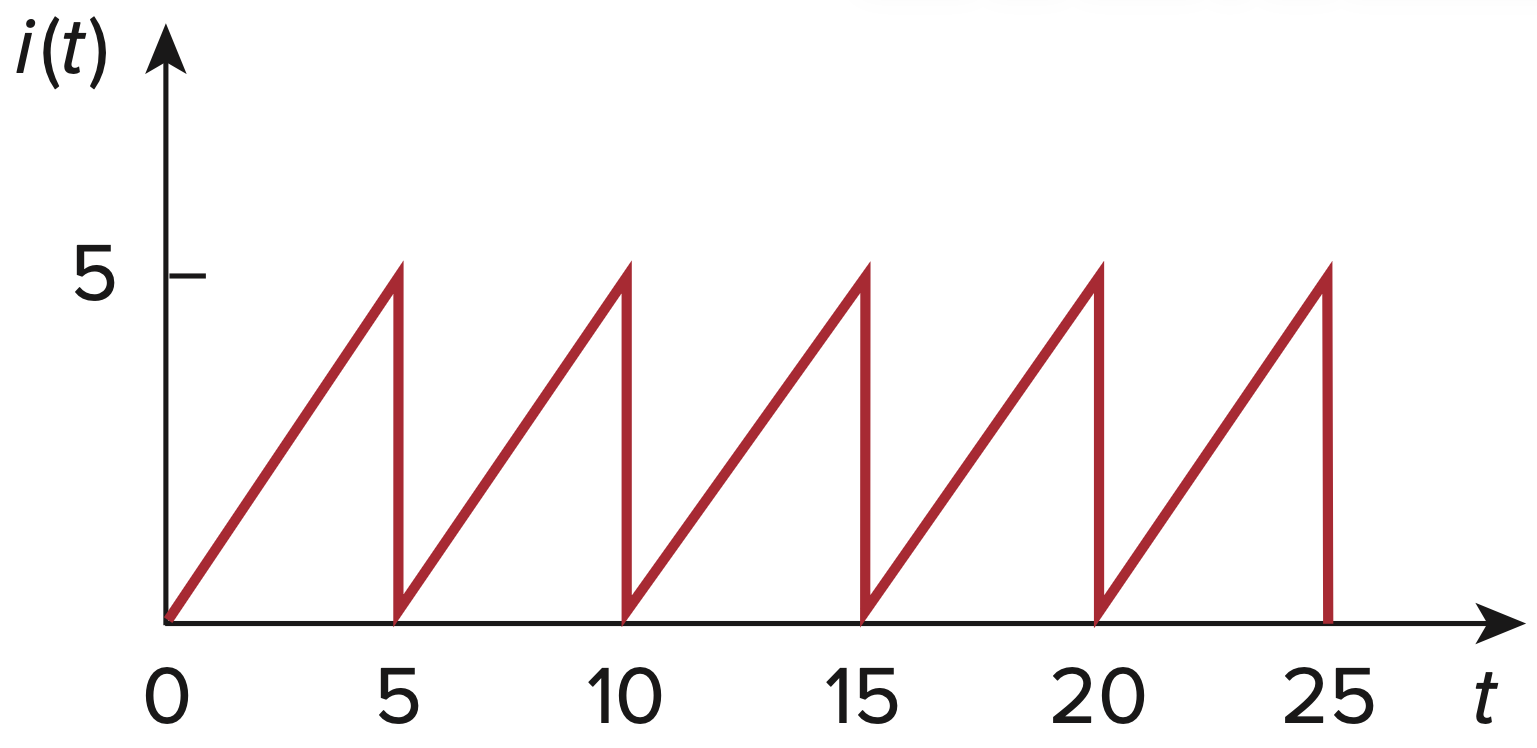
\includegraphics[width=0.7\textwidth]{figures/rms.png}
\end{exercise}

\ifshowsolutions
\begin{solution}
The waveform is a sawtooth with peak value 5 A and period \(T = 5\,\text{s}\):
\[
I = \sqrt{\frac{1}{T} \int_0^T i^2(t) dt} = \sqrt{\frac{1}{5} \int_0^5 \left(\frac{5t}{5}\right)^2 dt} = \sqrt{\frac{1}{5} \cdot \frac{1}{3} \cdot (5^3 - 0^3)}\,\text{A} \approx 2.89\,\text{A}
\]
\end{solution}
\fi

% ----- Exercise 4 -----
\begin{exercise}[Peak Phasors]
For the following signals, find the complex amplitudes corresponding to a cosine reference as well as the rectangular form of the phasors.
\begin{enumerate}[label=\alph*)]
  \item $v(t) = 21 \cos(4t - 15^{\circ})\,\text{V}$
  \item $i(t) = -8 \sin(10t + 70^{\circ})\,\text{mA}$
\end{enumerate}
\end{exercise}

\ifshowsolutions
\begin{solution}
\begin{enumerate}[label=\alph*)]
\item Peak phasor (cosine reference):
\[
\underline{\hat{v}} = 21 \angle -15^{\circ}\,\text{V}
\]
Rectangular form:
\[
\underline{\hat{v}} = 21 \left(\cos(-15^{\circ}) + j \sin(-15^{\circ})\right)\,\text{V} \approx (20.28 - j5.44)\,\text{V}
\]
\item Convert to cosine form:
\[
i(t) = -8 \sin(10t + 70^{\circ})\,\text{mA} = 8 \sin(10t + 250^{\circ})\,\text{mA} = 8 \cos(10t + 160^{\circ})\,\text{mA}
\]
Peak phasor (cosine reference):
\[
\underline{\hat{i}} = 8 \angle 160^{\circ}\,\text{mA}
\]
Rectangular form:
\[
\underline{\hat{i}} = 8 \left(\cos(160^{\circ}) + j \sin(160^{\circ})\right)\,\text{mA} \approx (-7.52 + j2.74)\,\text{mA}
\]
\end{enumerate}
\end{solution}
\fi

% ----- Exercise 5 -----
\begin{exercise}[Phasor Arithmetic]
Two voltages $v_1$ and $v_2$ appear in series so that their sum is $v = v_1 + v_2$.

If $v_1 = 10\cos(50t - \frac{\pi}{3})\,\text{V}$ and $v2 = 12\cos(50t + 30^{\circ})\,\text{V}$, find $v$.
\end{exercise}

\ifshowsolutions
\begin{solution}
Convert both to phasors:
\[
\underline{\hat{v}}_1 = 10 \angle -60^{\circ}\,\text{V}, \quad \underline{\hat{v}}_2 = 12 \angle 30^{\circ}\,\text{V}
\]
Convert to rectangular form:
\[
\underline{\hat{v}}_1 = 10 \left(\cos(-60^{\circ}) + j \sin(-60^{\circ})\right)\,\text{V} = (5 - j8.66)\,\text{V}
\]
\[
\underline{\hat{v}}_2 = 12 \left(\cos(30^{\circ}) + j \sin(30^{\circ})\right)\,\text{V} = (10.39 + j6)\,\text{V}
\]
Sum the phasors:
\[
\underline{\hat{v}} = \underline{\hat{v}}_1 + \underline{\hat{v}}_2 = ((5 + 10.39) + j(-8.66 + 6))\,\text{V} = (15.39 - j2.66)\,\text{V}
\]
Convert back to polar form:
\[
|\underline{\hat{v}}| = \sqrt{15.39^2 + (-2.66)^2}\,\text{V} \approx 15.62\,\text{V}
\]
\[
\theta = \tan^{-1}\left(\frac{-2.66}{15.39}\right) \approx -9.8^{\circ}
\]
Thus:
\[
\underline{\hat{v}} = 15.62 \angle -9.8^{\circ}\,\text{V}
\]
Convert back to time domain:
\[
v(t) = 15.62 \cos(50t - 9.8^{\circ})\,\text{V}
\]
\end{solution}
\fi

% ----- Exercise 6 -----
\begin{exercise}[AC Circuit]
A series $RLC$ circuit has $R = 80\,\Omega$, $L = 240\,\text{mH}$, and $C = 5\,\text{mF}$.

If the input voltage is $v(t) = 10\cos(2t)\,\text{V}$, find the current flowing through the circuit.
\end{exercise}

\ifshowsolutions
\begin{solution}
Angular frequency:
\[
\omega = 2\,\text{rad/s}
\]
Impedances:
\[
\underline{Z}_R = 80\,\Omega
\]
\[
\underline{Z}_L = j\omega L = (j2 \cdot 0.24)\,\Omega = j0.48\,\Omega
\]
\[
\underline{Z}_C = \frac{1}{j\omega C} = \frac{1}{j2 \cdot 0.005}\,\Omega = -j100\,\Omega
\]
Total impedance:
\[
\underline{Z} = \underline{Z}_R + \underline{Z}_L + \underline{Z}_C = 80\,\Omega + j0.48\,\Omega - j100\,\Omega = (80 - j99.52)\,\Omega
\]
Magnitude and phase of total impedance:
\[
|\underline{Z}| = \sqrt{80^2 + (-99.52)^2}\,\Omega \approx 127.69\,\Omega
\]
\[
\theta_Z = \tan^{-1}\left(\frac{-99.52}{80}\right) \approx -51.21^{\circ}
\]
Phasor form of voltage:
\[
\underline{\hat{v}} = 10 \angle 0^{\circ}\,\text{V}
\]
Phasor form of current:
\[
\underline{\hat{i}} = \frac{\underline{\hat{v}}}{\underline{Z}} = \frac{10 \angle 0^{\circ}\,\text{V}}{127.69 \angle -51.21^{\circ}\,\Omega} = \frac{10\,\text{V}}{127.69 \exp(-j51.21^{\circ})\,\Omega} \approx 78.3 \angle 51.21^{\circ}\,\text{mA}
\]
Convert back to time domain:
\[
i(t) = 78.3 \cos(2t + 51.21^{\circ})\,\text{mA}
\]
\end{solution}
\fi

% ----- Exercise 7 -----
\begin{exercise}[Equivalent Impedance]
Given the AC network with  $R_1 = 10\,\Omega$, $R_2 = 20\,\Omega$, $L = 50\,\mathrm{mH}$, $C = 100\,\mu\mathrm{F}$, $\omega = 1000\,\mathrm{rad/s}$:

\begin{center}
\begin{circuitikz}[european, scale=1]
  \draw
  % Eingang
  (0,0) node[left]{A}
  to[R=$R_1$] (3,0)

  % Parallelschaltung
  (3,0) -- (3,2)
  to[L=$L$] (6,2)
  -- (6,0)

  (3,0) -- (3,-2)
  to[C=$C$] (6,-2)
  -- (6,0)

  % R2
  to[R=$R_2$] (9,0)
  node[right]{B};
\end{circuitikz}
\end{center}

Determine:

\begin{enumerate}
  \item the complex impedances of the individual components,
  \item the complex equivalent impedance between terminals A and B,
  \item the magnitude and phase of the equivalent impedance.
\end{enumerate}
\end{exercise}

\ifshowsolutions
\begin{solution}
\[
\underline{Z}_R = R
\]
\[
\underline{Z}_L = j \omega L = j \cdot 1000 \cdot 0.05 = j50\,\Omega
\]
\[
\underline{Z}_C = \frac{1}{j \omega C} = \frac{1}{j \cdot 1000 \cdot 100 \cdot 10^{-6}} = -j10\,\Omega
\]
\[
\underline{Z}_{LC} = \left( \frac{1}{Z_L} + \frac{1}{Z_C} \right)^{-1} = \frac{1}{j0.08} = -j12.5\,\Omega
\]
\[
\underline{Z} = R_1 + Z_{LC} + R_2 = (30 - j12.5)\,\Omega
\]
\[
|\underline{Z}| = \sqrt{30^2 + 12.5^2} \approx 32.5\,\Omega
\]
\[
\varphi = \arctan\left(\frac{-12.5}{30}\right) \approx -22.6^\circ
\]
\end{solution}
\fi

% ----- Exercise 8 -----
\begin{exercise}[Equivalent Admittance]
Determine the admittance \underline{Y} for the circuit shown below.

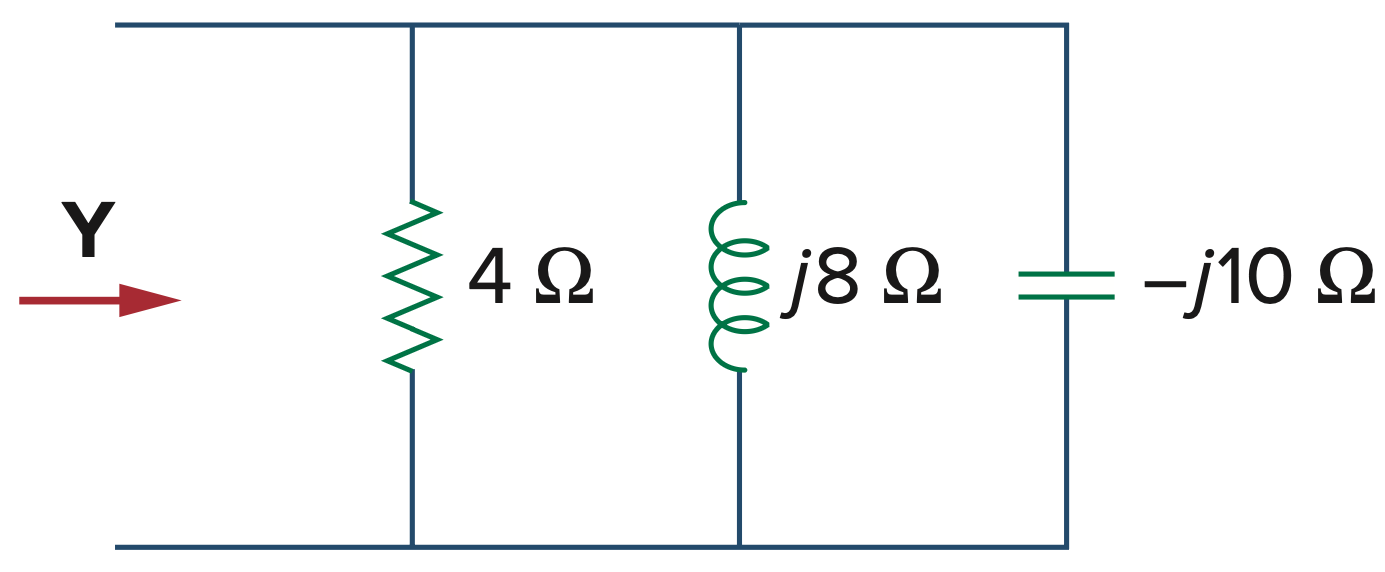
\includegraphics[width=0.7\textwidth]{figures/admittance.png}
\end{exercise}

\ifshowsolutions
\begin{solution}
Calculate the individual admittances:
\[
\underline{Y}_R = \frac{1}{\underline{Z}_R} = \frac{1}{4\,\Omega} = 0.25\,\text{S}
\]
\[
\underline{Y}_L = \frac{1}{\underline{Z}_L} = \frac{1}{j8\,\Omega} = -j0.125\,\text{S}
\]
\[
\underline{Y}_C = \frac{1}{\underline{Z}_C} = \frac{1}{-j10\,\Omega} = j0.1\,\text{S}
\]
Total admittance:
\[
\underline{Y} = \underline{Y}_R + \underline{Y}_L + \underline{Y}_C = 0.25\,\text{S} - j0.125\,\text{S} + j0.1\,\text{S} = (250 - j25)\,\text{mS}
\]
\end{solution}
\fi

% ----- Exercise 9 -----
\begin{exercise}[$RLC$ Circuit]
Find $v(t)$ in the circuit below.

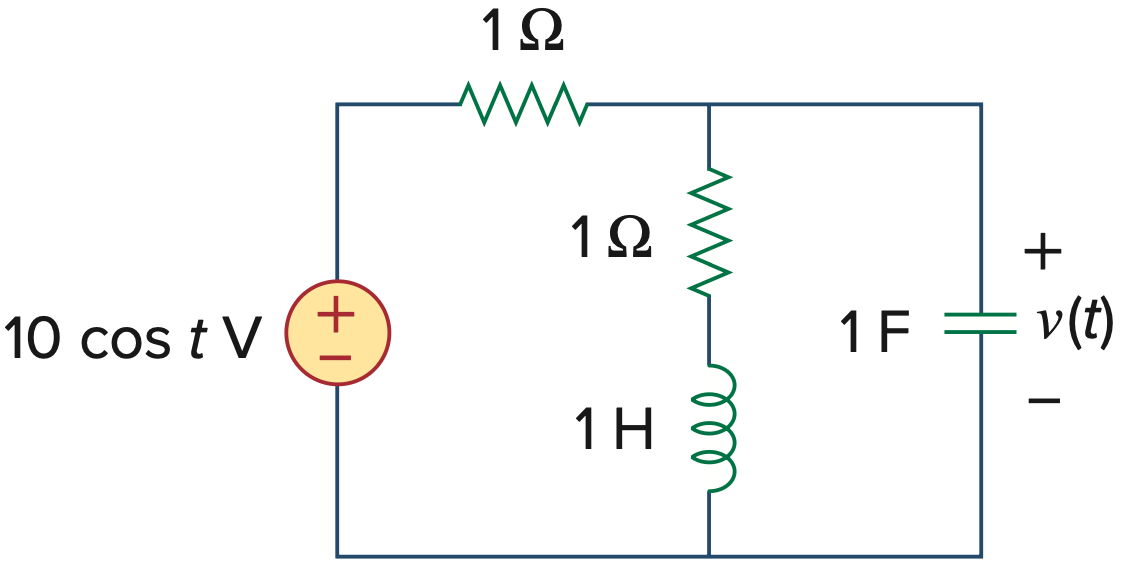
\includegraphics[width=0.7\textwidth]{figures/ACcircuit1.png}
\end{exercise}

\ifshowsolutions
\begin{solution}
We are given the time-domain source
\[
v_s(t) = 10\cos t\,\text{V}.
\]
In complex (exponential) representation we write this as the real part of a complex exponential:
\[
v_s(t) = Re(\underline{\hat{v}}_s e^{j\omega t}),\qquad \underline{\hat{v}}_s = 10,\ \omega=1\ \text{rad/s},
\]
so \(v_s(t)=Re(10 e^{j t})\).

At \(\omega=1\),
\[
\underline{Z}_{R_1} = 1,\qquad \underline{Z}_{R_2} = 1,\qquad \underline{Z}_L = j\omega L = j,\qquad \underline{Z}_C = \frac{1}{j\omega C} = -j.
\]

The series \(R_2\!-\!L\) branch impedance is
\[
\underline{Z}_{RL}=1+j.
\]

The parallel combination of \(\underline{Z}_{RL}\) and \(\underline{Z}_C\) has admittance
\[
\underline{Y}_{p} = \frac{1}{\underline{Z}_{RL}} + \frac{1}{\underline{Z}_C} = \frac{1}{1+j} + \frac{1}{-j}.
\]
Compute each term explicitly:
\[
\frac{1}{1+j} = \frac{1-j}{(1+j)(1-j)} = \frac{1-j}{2} = \tfrac12 - \tfrac12 j,
\qquad
\frac{1}{-j} = j.
\]
Thus
\[
\underline{Y}_p = \left(\tfrac12 - \tfrac12 j\right) + j = \tfrac12 + \tfrac12 j.
\]
Therefore the equivalent impedance of the parallel network is
\[
\underline{Z}_p = \frac{1}{\underline{Y}_p} = \frac{1}{\tfrac12 + \tfrac12 j} = \frac{\tfrac12 - \tfrac12 j}{(\tfrac12)^2 + (\tfrac12)^2} = 1-j.
\]

The total series impedance seen by the source is
\[
\underline{Z}_{\text{tot}} = \underline{Z}_{R_1} + \underline{Z}_p = 1+(1-j) = 2-j.
\]

Now form the complex current \(\underline{\hat{i}}\) (the complex amplitude multiplying \(e^{j t}\)) by dividing the complex source amplitude by the complex impedance:
\[
\underline{\hat{i}} = \frac{\underline{\hat{v}}_s}{\underline{Z}_{\text{tot}}} = \frac{10}{2-j}.
\]
Perform the algebraic division by multiplying numerator and denominator by the conjugate:
\[
\underline{\hat{i}} = 10\frac{2+j}{(2-j)(2+j)} = 10\frac{2+j}{5} = 4+2j.
\]
Thus the complex current amplitude is \(\underline{\hat{i}} = 4+2j\). (Its magnitude is \(|\underline{\hat{i}}| = \sqrt{4^2+2^2} \approx 4.472\) and its angle \(\arg(\underline{\hat{i}}) = \arctan(2/4) = 26.57^\circ\), if one prefers polar form.)

The complex voltage across the parallel network (and thus across the capacitor) is
\[
\underline{\hat{v}}_p = \underline{\hat{i}}\,\underline{Z}_p = (4+2j)(1-j).
\]
Multiply out:
\[
\underline{\hat{v}}_p = 4(1-j)+2j(1-j) = 4-4j+2j-2j^2 = 4-2j+2 = 6-2j.
\]
So the complex amplitude of the capacitor voltage is \(\underline{\hat{v}}_p = 6-2j\).

We may express this two ways:

\textbf{(a) Time-domain real part of the exponential:}
\[
v(t) = Re(\underline{\hat{v}}_p e^{j t}) = Re((6-2j)e^{j t}).
\]
Expanding \((6-2j)e^{jt} = (6-2j)(\cos t + j\sin t)\) and taking the real part gives
\[
v(t) = 6\cos t + 2\sin t.
\]

\textbf{(b) Amplitude–phase form:} compute magnitude and angle of \(\underline{\hat{v}}_p\):
\[
|\underline{\hat{v}}_p| = \sqrt{6^2+(-2)^2} \approx 6.325,
\]
\[
\arg(\underline{\hat{v}}_p) = \arctan\!\bigg(\frac{-2}{6}\bigg) \approx -18.43^\circ.
\]
Thus
\[
\underline{\hat{v}}_p = 6.325\angle(-18.43^\circ),
\]
and therefore
\[
v(t) = 6.325\cos\big(t-18.43^\circ\big)\,\text{V},
\]
which is algebraically equivalent to \(v(t) = 6\cos t+2\sin t\).
\end{solution}
\fi

% ----- Exercise 10 -----
\begin{exercise}[Phase-shifted Source Current]
Determine the value of $i_s(t)$ in the circuit below.

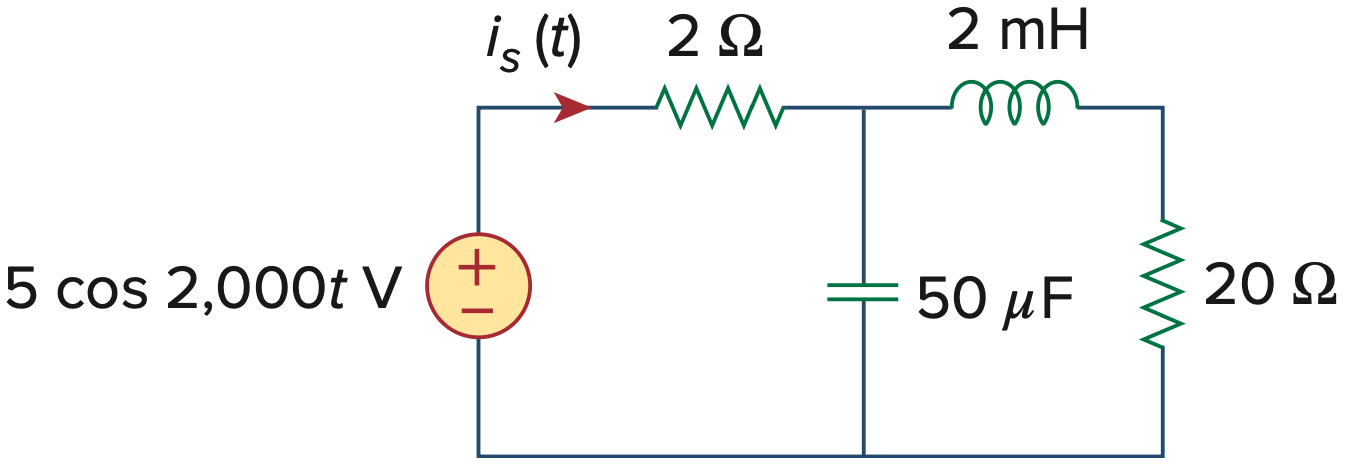
\includegraphics[width=0.7\textwidth]{figures/ACcircuit2.png}
\end{exercise}

\ifshowsolutions
\begin{solution}
\[
\omega = 2000\;\text{rad/s}
\]

\[
\underline{Z}_C = \frac{1}{j \omega C} = \frac{-j}{2000 \cdot 50 \times 10^{-6}}\,\Omega = -j 10\,\Omega
\]

\[
\underline{Z}_{RL} = 20 + j \omega L = (20 + j 2000 \cdot 2 \times 10^{-3})\,\Omega = (20 + j 4)\,\Omega
\]

\[
\underline{Y}_p = \frac{1}{\underline{Z}_C} + \frac{1}{Z_{RL}} = j 0.1 + \frac{1}{20 + j 4} = j 0.1 + \frac{20 - j 4}{416} = \left(\frac{20}{416} + j \frac{37.6}{416}\right)\,\text{S}
\]

\[
\underline{Z}_p = \frac{1}{\underline{Y}_p} = \left(\frac{\frac{20}{416} - j \frac{37.6}{416}}{(\frac{20}{416})^2 + (\frac{37.6}{416})^2}\right)\,\Omega = (4.58716 - j 8.62385)\,\Omega
\]

\[
\underline{Z}_{\text{tot}} = \underline{Z}_{R_2} + Z_p = 2\,\Omega + (4.58716 - j8.62385)\,\Omega = (6.58716 - j 8.62385)\,\Omega
\]

\[
\underline{\hat{i}}_s = \frac{\underline{\hat{v}}_s}{\underline{Z}_{\text{tot}}} = \frac{5}{6.58716 - j 8.62385}\,\text{A} = (0.27714 + j 0.36949)\,\text{A}
\]

\[
\hat{i}_s = \sqrt{(0.27714)^2 + (0.36949)^2}\,\text{A} = 0.460753\,\text{A}
\]

\[
\varphi_{i_s} = \tan^{-1}\!\left(\frac{0.36949}{0.27714}\right) = 52.6263^\circ
\]

\[
i_s(t) = 460.7 \cos\!\left(2000t + 52.63^\circ\right)\,\text{mA}
\]
\end{solution}
\fi

\end{document}